\subsection{Definitionen und wichtige Eigenschaften}
In diesem Abschnitt definieren wir den numerischen Wertebereich und den numerischen Radius für linear, beschränkte Operatoren in einem Hilbertraum. Wir orientieren uns dabei stark an den ersten Kapiteln aus \parencite[][Kapitel 1,2]{gustafson1997numerical}. Falls nicht anders erwähnt sei $\mathcal{H}$ ein komplexer Hilbertraum und $ T \in \mathcal{L} (\mathcal{H}) $ für den gesamten Abschnitt.

\begin{definition}[Numerischer Wertebereich]
	 Die Menge 
	\begin{align*}
		W(T) := \{ \left< Tx,x \right> \; | \; x \in \mathcal{H},\; ||x||=1 \}
	\end{align*}
	heißt der numerische Wertebereich von $T$.
\end{definition}

Einige elementare Eigenschaften werden in folgender Proposition festgehalten:

\begin{prop} \label{prop:properties_numran}
	Für $W(T)$ gilt:
	\begin{enumerate}[label=(\roman*)]
		\item \label{prop:prop_numran_lin} für alle $a , b \in \mathbb{C}$ gilt: $W( aI + b T) = a + b W(T)$
		\item $W(T)$ ist konjugiert symmetrisch, d. h. $W(T^*) =  \{\overline{\omega} \; | \; \omega \in W(T)\}$
		\item $W(T)$ ist invariant unter Ähnlichkeitstransformationen mit unitären Operatoren, d. h. für alle unitären Operatoren $U \in \mathcal{L}(\mathcal{H})$ gilt: $W(U^*TU)=W(T)$
	\end{enumerate}
\end{prop}

\begin{proof}
	\begin{enumerate}[label= (\roman*)]
		\item Seien $a, b \in \mathbb{C}$. Dann folgt sofort:
		\begin{align}
			W(a I + b T) & = \{ \left< (a I + b T)x,x \right> \; | \; x \in \mathcal{H},\; ||x||=1 \} \nonumber \\
			& = \{ a \left< Ix,x \right> + b \left< Tx,x \right> \; | \; x \in \mathcal{H},\; ||x||=1 \} \nonumber \\
			& = \{ a ||x||^2 + b \left< Tx,x \right> \; | \; x \in \mathcal{H},\; ||x||=1 \} \nonumber \\
			& = a+ b W(T)
		\end{align} 
		\item Sei $T^*$ der zu $T$ konjugierte Operator. Dann folgt unter Ausnutzung der Definition von $T^*$ für den numerischen Wertebereich von $T^*$:
		\begin{align}
			W(T^*) & = \{ \left< T^*x,x \right> \; | \; x \in \mathcal{H},\; ||x||=1 \} \nonumber \\
				& = \{ \left< x,Tx \right> \; | \; x \in \mathcal{H},\; ||x||=1 \} \nonumber \\
				& = \{ \overline{ \left< Tx,x \right> } \; | \; x \in \mathcal{H},\; ||x||=1 \} \nonumber \\
				& = \{ \overline{\omega}, \omega \in W(T)\ \}
		\end{align}
		\item Sei $U \in \mathcal{L}(\mathcal{H})$ ein unitärer Operator, das heißt, es gilt $U^*U = UU^*=I$. Damit folgt direkt:
		\begin{align}
			W(U^*TU) & = \{ \left< U^*TUx,x \right> \; | \; x \in \mathcal{H},\; ||x||=1 \} \nonumber \\
				& = \{ \left< TUx,Ux \right> \; | \; x \in \mathcal{H},\; ||x||=1 \} \nonumber \\
				\text{ \tiny ($U$ unitär)} &= \{ \left< Ty,y \right> \; | \; y \in \mathcal{H},\; ||y||=1 \} \nonumber \\
				& = W(T)
		\end{align}
	\end{enumerate}
\end{proof}

\begin{ex} \label{ex:num_ran}
	\begin{enumerate}[label=(\roman*)]
		\item \label{ex:ev_zero} Sei $H=\mathbb{C}^2$. Wir betrachten die Matrix 
		\begin{align*}
			A = \begin{pmatrix}
				0 & 1 \\
				0 & 0
			\end{pmatrix}
		\end{align*}
		Nun zeige man, dass $W(A)= \{ z \in \mathbb{C} \;  | \; |z| \le \frac{1}{2} \} =: B_\frac{1}{2}$.
		\begin{enumerate}[label=]
			\item $"\subseteq"$ Sei $z\in W(A)$. Dann existiert ein $x=(x_1, x_2) \in \mathbb{C}^2 \text{ mit } \|x\|^2= |x_1|^2 + |x_2|^2=1$ und
			\begin{align}
				|z|&=|\left< Ax,x \right>| = |x_2\overline{x_1}|= |x_2||x_1| \nonumber \\
				& = \frac{1}{2} \left[|x_1|^2 + 2|x_1||x_2| +|x_2|^2 - |x_1|^2 - |x_2|^2 \right] \nonumber \\
				& = \frac{1}{2} \left[|x_1|^2 +|x_2|^2 - |x_1|^2 + 2|x_1||x_2| -|x_2|^2 \right] \nonumber \\
				& =  \frac{1}{2} \left[|x_1|^2 +|x_2|^2 - (|x_1| -|x_2|)^2 \right] \nonumber \\
				& \le \frac{1}{2} \left[|x_1|^2 +|x_2|^2 \right] \nonumber \\
				& = \frac{1}{2}
			\end{align} 
			Also $z \in B_\frac{1}{2}$
			\item $"\supseteq"$ Sei $z \in B_\frac{1}{2}$. Dann lautet die Darstellung in Polarkoordinaten: $z=re^{i\phi}$ mit $0 \le r \le \frac{1}{2}$ und $\phi \in \mathbb{R}$. Wählt man nun $x=(\cos \alpha, e^{i\phi}\sin \alpha) \in \mathbb{C}^2$, wobei $\alpha$ so gewählt wird, dass $\sin 2\alpha = 2r$, dann ist \[ \| x\|^2=\cos^2 \alpha + |e^{i\phi}|\sin^2 \alpha=1 \] und mithilfe der bekannten Additionstheoreme für den Sinus
			\begin{align}
				\left< Ax,x \right> &= e^{i\phi}\sin \alpha \cos \alpha = \frac{1}{2} e^{i\phi} \sin 2\alpha = re^{i\phi} = z
			\end{align}
			Also $z \in W(A)$.
		\end{enumerate}

		\item Unter Ausnutzung der Eigenschaften vom numerischen Wertebereich aus Proposition \ref{prop:properties_numran} und dem vorherigen Beispiel \ref{ex:ev_zero}, folgt für beliebige $a \in \mathbb{C}$ und 
		\begin{align*}
			A = \begin{pmatrix}
				0 & a \\
				0 & 0
			\end{pmatrix},
		\end{align*}
		dass $W(A)= \{ z \in \mathbb{C} \;  | \; |z| \le \frac{|a|}{2} \}$

		\begin{figure}[H]
			\caption{Numerischer Wertebereich für den Fall $a=2$}
			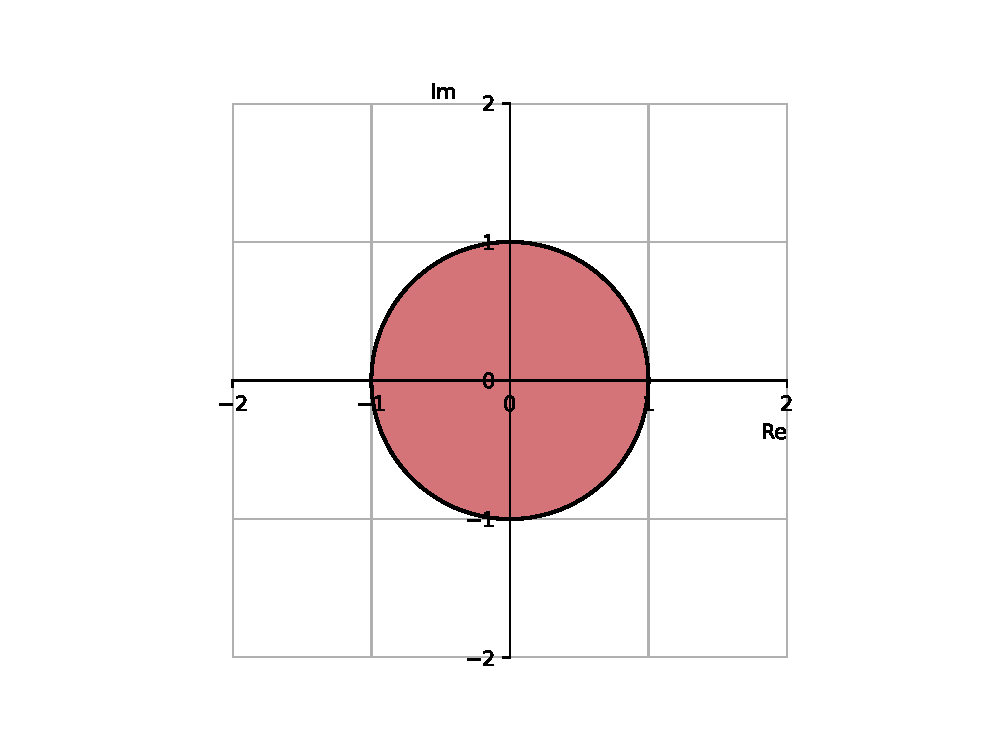
\includegraphics{circle.eps}
		\end{figure}
	\end{enumerate}
	
\end{ex}

Im Zweidimensionalen bildet das sogenannte Ellipsenlemma \parencite[S. 3ff]{gustafson1997numerical} eine schöne geometrische Darstellung des numerischen Wertebereichs. Für den Beweis wird ein kleines technisches Lemma benötigt, das durch eine direkte Rechnung bewiesen werden kann:

\begin{lem} \label{lem:hlem_ellipse}
	Sei $A$ eine quadratische, komplexe Matrix in $\mathit{Mat}_{n,n}(\mathbb{C})$, $n\in \mathbb{N}$, $\gamma \in \mathbb{R}$ und die Matrix $C$ definiert als
	\begin{align*}
		C := \frac{1}{2} \bigg[ (A+A^*)+\gamma(A-A^*) \bigg].
	\end{align*}
	Dann gilt für die numerischen Wertebereiche von A und C folgende Beziehung:
	\begin{align*}
		a+ib=\omega \in W(A) \iff a+ i \gamma b= \widetilde{\omega} \in W(C) \\
		\text{mit }  a, b \in \mathbb{R}
	\end{align*}
\end{lem}

\begin{proof}
	$"\Rightarrow"$ Sei $a+ib=\omega \in W(A) \; , \; a, b \in \mathbb{R}$. Dann existiert ein $x \in \mathbb{C}^n$ mit $\|x\|=$ und $\left< Ax,x \right>=\omega$. Damit folgt über eine direkte Berechnung und Proposition \ref{prop:properties_numran}:
	\begin{align} \label{eq:hlem_ellipse_hin}
		\left< Cx,x \right> & = \left< \frac{1}{2} \bigg[ (A+A^*)+\gamma(A-A^*) \bigg] x, x \right> \nonumber \\
		& = \frac{1}{2} \bigg[ \left< Ax,x \right> + \gamma \left< Ax,x \right> + \left< A^*x,x \right> - \gamma \left< A^*x,x \right> \bigg] \nonumber \\
		& = \frac{1}{2} \biggl[ \omega + \gamma \omega + \overline{\omega} - \gamma \overline{\omega} \biggr] \nonumber \\
		& = a + i \gamma b \nonumber \\ 
		&= \widetilde{\omega}
	\end{align}
	Also $\widetilde{\lambda} \in W(C)$. \\

	$"\Leftarrow"$ Sei nun $a+i \gamma b=\widetilde{\omega} \in W(C) \; , \; a, b \in \mathbb{R}$. Dann existiert ein\mbox{ $y \in \mathbb{C}^n \; , \; \| y \| = 1$ } mit $\left< Cy,y \right>= \widetilde{\omega}$. Mithilfe von Gleichung (\ref{eq:hlem_ellipse_hin}) folgt:
	\begin{align}
		\left< Cy,y \right> & = \frac{1}{2} \bigg[ \left< Ay,y \right> + \gamma \left< Ay,y \right> + \left< A^*y,y \right> - \gamma \left< A^*y,y \right> \bigg] \nonumber \\
		& = \operatorname{Re} \left< Ay,y \right> + \gamma \operatorname{Im} \left< Ay,y \right> 
	\end{align}
	Also $\left< Ay,y \right> = a +ib = \omega$ und damit $\omega \in W(A)$.

\end{proof}

Nun lässt sich das Ellipsenlemma \parencite[vgl. S. 3f]{gustafson1997numerical} beweisen. Im Gegensatz zum Beweis aus \parencite{gustafson1997numerical} wird ein eleganterer Weg nach \parencite{li1996simple_ellipse} gewählt, denn dieser nutzt geschickt die Eigenschaften des numerischen Wertebereich aus Proposition \ref{prop:properties_numran} aus.

\begin{lem}[Ellipsenlemma] \label{lem:ell_lem}
	Sei $A$ linear, beschränkter Operator auf einem zweidimensionalen Hilbertraum $\mathcal{G}$. Dann ist $W(A)$ eine Ellipse, dessen Brennpunkte genau die Eigenwerte von A sind.
\end{lem}
\begin{proof}
	Sei $A$ linear und beschränkt in $Mat_{2,2}(\mathbb{C})$. Wendet man die Schur-Zerlegung auf $A$ an, dann existieren eine unitäre Matrix U und eine obere Dreiecksmatrix D, sodass $A=U^*DU$ bzw. $D=UAU^*$. Nach Proposition \ref{prop:properties_numran}(iii) haben $A$ und $U$ denselben numerischen Wertebereich, daher wird im folgenden o. B. d. A. angenommen, dass A eine obere Dreiecksmatrix ist. Man wähle nun als Darstellung:
	\begin{align*}
		A = \begin{pmatrix}
			\lambda_1 & a\\ 
			0 & \lambda_2
		\end{pmatrix} .
	\end{align*} 
	\begin{enumerate}[label=\protect\circled{\arabic*}]
		\item Falls $\lambda_1=\lambda_2 = 0$, dann ist $W(A)= \{ z \in \mathbb{C} \;  | \; |z| \le \frac{|a|}{2} \}$ ein Kreis nach Beispiel \mbox{ \ref{ex:num_ran} \ref{ex:ev_zero} }. Dieser kann auch als Ellipse mit Brennpunkt 0 betrachtet werden.
		\item Betrachtet man nun den Fall $a=0$, dann ist 
		\begin{align}
			W(A) & = \{ \left< Ax,x \right> \; | \; (x_1, x_2)=x \in \mathcal{G},\; \|x\|=1 \} \nonumber \\
			& = \{ \lambda_1 |x_1|^2 + \lambda_2 |x_2|^2 \; | \; (x_1, x_2)=x \in \mathcal{G},\; \|x\|^2=|x_1|^2+|x_2|^2=1 \} \nonumber \\
			& = \{ \lambda_1 |x_1|^2 + \lambda_2 (1-|x_1|^2) \; | \; (x_1, x_2)=x \in \mathcal{G},\; \|x\|^2=|x_1|^2+|x_2|^2=1 \} \nonumber \\
			& = \{ \lambda_1 t + \lambda_2 (1-t)  \; | \; 0 \le t \le 1 \}
		\end{align}
		die Strecke zwischen $\lambda_1$ und $\lambda_2$, welche als degenerierte Ellipse mit Brennpunkten $\lambda_1$ und $\lambda_2$ betrachtet werden kann.
		\item Zuletzt wird der allgemeine Fall $\lambda_1, \lambda_2 \neq 0$ und $a \neq 0$ betrachtet. Um den numerischen Wertebereich von A zu bestimmen, werden zunächst einige Verschiebungen und Transformationen untersucht, die zu bereits bekannten Ergebnissen führen. Man definiere 
		\begin{align*}
			B &:= A - \frac{\lambda_1+\lambda_2}{2} = \begin{pmatrix}
				\frac{\lambda_1-\lambda_2}{2} & a \\
				0 & - \frac{\lambda_1-\lambda_2}{2}
			\end{pmatrix} =: \begin{pmatrix}
				\lambda & a \\
				0 & - \lambda
			\end{pmatrix} \\
			C &:= \frac{1}{2} \bigg[ (B+B^*)+\gamma(B-B^*) \bigg] = \frac{1}{2}\begin{pmatrix}
				2\lambda & a+ \gamma a \\
				a - \gamma a & -2\lambda 
			\end{pmatrix}
		\end{align*}
		Wählt man nun geschickt $\gamma=2\frac{\sqrt{\lambda^2+\frac{a^2}{4}}}{a}$, dann vereinfacht sich die Matrix $C$ zu:
		\begin{align*}
			C = \begin{pmatrix}
				\lambda & \frac{a}{2}+ \sqrt{\lambda^2+\frac{a^2}{4}}  \\
				\frac{a}{2}- \sqrt{\lambda^2+\frac{a^2}{4}} & - \lambda  
			\end{pmatrix}
		\end{align*}
		Dann hat $C$ den doppelten Eigenwert 0, denn:
		\begin{align}
			\det(C - \mu) = -(\lambda^2-\mu^2) - (\frac{a^2}{4}-(\lambda^2+\frac{a^2}{4})) = -\mu^2  \overset{!}{=} 0 \nonumber \\
			\iff \mu_{1,2} = 0
		\end{align}
		Damit lässt sich $C$ mithilfe einer Schur-Zerlegung in eine unitär ähnliche obere Dreiecksmatrix überführen. Eine langwierige Rechnung zeigt:
		\[ \widetilde{C} := \begin{pmatrix}
			0 & 2\sqrt{\lambda^2+\frac{a^2}{4}} \\
			0 & 0
		\end{pmatrix}.\] \\ 
		Dann ist 
		\begin{align} \label{eq:numran_c}
			W(\widetilde{C})=W(C)=\{ x+iy=\widetilde{z} \in \mathbb{C} \; | \; x^2 + y^2 \le r^2 \}	
		\end{align}
		nach dem ersten Fall ein Kreis um den Ursprung.mit Radius $r := \sqrt{\lambda^2+\frac{a^2}{4}}$. Nach dem vorigen Hilfslemma \ref{lem:hlem_ellipse} gilt nun:
		\begin{align*}
			x+iy=\widetilde{z} \in W(C) & \overset{Lemma}{\underset{\ref{lem:hlem_ellipse}}{\iff}} x+i{y}\frac{1}{\gamma}=z \in W(B)  \\
			& \overset{(\ref{eq:numran_c})}{\iff} W(B)=\{ x+iy=z \in \mathbb{C} \; | \; x^2 + \gamma^2y^2 \le r^2\} \\
			& \iff W(B)=\{ x+iy=z \in \mathbb{C} \; | \; \frac{x^2}{r^2} + \frac{\gamma^2y^2}{r^2} \le 1\}
		\end{align*}
		$W(B)$ ist also eine Ellipse mit Ursprung 0 und großer Halbachse $s_1=r$ und kleiner Halbachse $s_2=\frac{r}{\gamma}$. Nun lassen sich die Brennpunkte $f_1$ und $f_2$ berechnen:
		\begin{align*}
			f_{1,2} = \pm \sqrt{s_1^2-s_2^2} = \pm \sqrt{r^2-\frac{r}{\gamma^2}^2} = \pm \sqrt{\lambda^2+\frac{a^2}{4}-\frac{a^2}{4}} = \pm \lambda 
		\end{align*}	
		(Die geometrischen Größen einer Ellipse sind im Anhang näher beschrieben.)\\\\	
		Die Brennpunkte sind genau die Eigenwerte $\lambda$ und $-\lambda$ von $B$. Um letztendlich den numerischen Wertebereich von A zu berechnen, nutze man die wieder Proposition \ref{prop:properties_numran}:
		\begin{align*}
			W(A) = W(B+\frac{\lambda_1+\lambda_2}{2}) \overset{Prop.}{\underset{\ref{prop:properties_numran}\ref{prop:prop_numran_lin}}{=}} W(B) + \frac{\lambda_1+\lambda_2}{2}
		\end{align*}
		Damit folgt, dass $W(A)$ eine Ellipse mit Brennpunkten $g_1=\lambda_1$ und $g_2=\lambda_2$ ist.
	\end{enumerate}
\end{proof}

\begin{rem}
	Es kann sogar gezeigt werden, dass für die kleine Halbachse der Ellipse gilt \parencite[vgl. S. 3f]{gustafson1997numerical}:
	\begin{align*}
		s_2 = \sqrt{ tr(A^*A) - |\lambda_1|^2 - |\lambda_2|^2 }
	\end{align*}
\end{rem}

\begin{ex}
	Sei 
	\begin{align*}
		A = \begin{pmatrix}
			-1 & 2 \\
			0 & 1
		\end{pmatrix}
	\end{align*}
	Dann ist $W(A)$ nach Lemma \ref{lem:ell_lem} eine Ellipse mit Brennpunkten 1 und -1.
	\begin{figure}[H]
		\caption{Numerischer Wertebereich von A}
		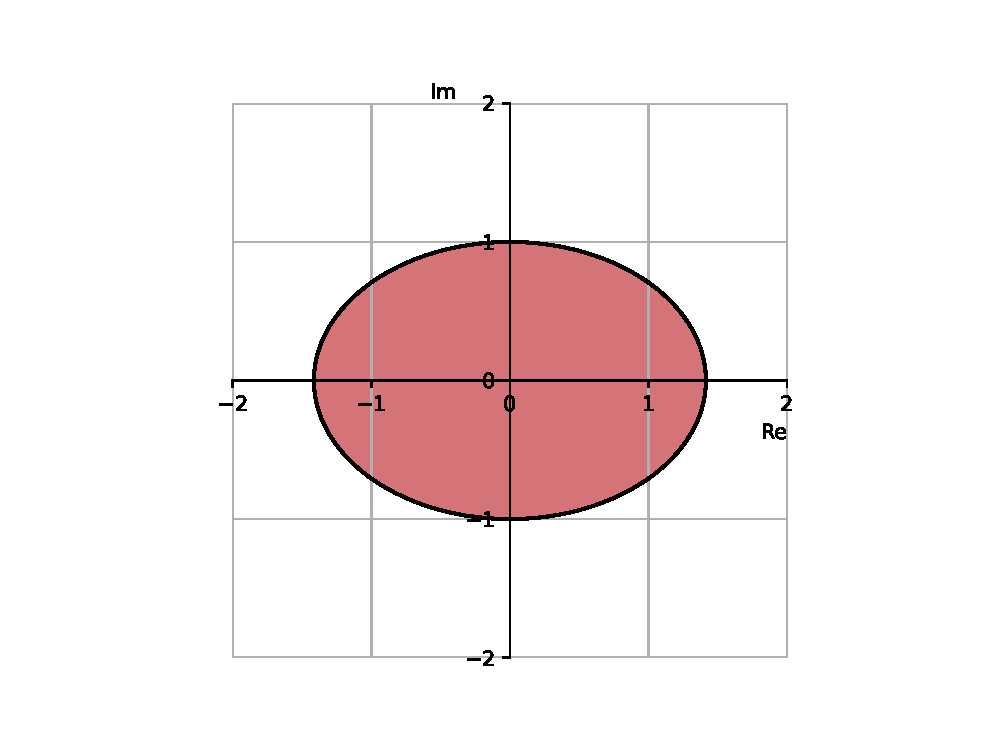
\includegraphics{ellipse.eps}
	\end{figure}
\end{ex}

Im Mehrdimensionalen gilt das Ellipsenlemma im Allgemeinen nicht, es kann aber gezeigt werden, dass der numerische Wertebereiche immer konvex ist. Diese Aussage wurde 1918 von O. Töplitz \parencite{Toeplitz1918} aufgestellt und ein Jahr später von F. Hausdorff bewiesen \parencite{Hausdorff1919}. Der Beweis wird nach \parencite[][S. 4]{gustafson1997numerical} geführt unter Zuhilfenahme von Anmerkungen aus \parencite[][Problem 210]{halmos2012hilbert}. Die Idee des Beweises besteht darin, einen gegebenen Operator in einem beliebigen Hilbertraum mithilfe einer geeigneten Transformation in einen Operator auf einen zweidimensionalen Hilbertraum zu überführen. Dann folgt die Aussage leicht mit dem Ellipsenlemma (Theorem \ref{lem:ell_lem}).

\begin{thm}[Töplitz-Hausdorff] \label{thm:toe_haus}
	Für $T \in \mathcal{L}(\mathcal{H})$ ist $W(T)$ konvex.
\end{thm} 
\begin{proof}
	Man wähle zwei beliebige Elemente aus dem numerischen Wertebereich von $T$. Seien also $\alpha, \beta \in W(T)$, das heißt es existieren Einheitsvektoren $x,y \in \mathcal{H}$ mit $\|x\|=\|y\|=1$, sodass $\alpha = \left< Tx,x \right>$ und analog $\beta = \left< Ty,y \right>$. Sei weiterhin $\gamma=t\alpha + (1-t)\beta \in W(T)$ für ein $t \in [0,1]$ eine beliebige Konvexkombination von von $\alpha$ und $\beta$. Dann ist zu zeigen: $\gamma \in W(T)$. Man definiere nun $V:=span \{x,y\}$. Falls $\dim V =1$, dann sind $x$ und $y$ linear abhängig. Es existiert also ein $s\in \mathbb{C}$ mit $x = sy$ mit $|s|=1$ und die Aussage folgt trivialerweise.

	Sei also $\dim V =2$. Man definiere nun die orthogonale Projektion (siehe Theorem \ref{thm_orth_proj}) $P$ von $\mathcal{H}$ auf $V$, dann gilt per Definition schon $Px=x$ und $Py=y$. Wir definieren den zweidimensionalen Operator 
	\begin{align*}
		T_P : V \longrightarrow V \\
		v \mapsto PTPv
	\end{align*}
	Da $P$ zusätzlich auch selbst-adjungiert ist, gilt nun:
	\begin{align}
		\left< T_Px,x \right> = \left< PTPx,x \right> = \left< Tx,Px \right> = \left< Tx,x \right> \\
		\left< T_Py,y \right> = \left< PTPy,y \right> = \left< Ty,Py \right> = \left< Ty,y \right>
	\end{align}
	Nach dem Ellipsenlemma \ref{lem:ell_lem} ist $W(T_P)$ eine Ellipse und damit konvex, also existiert ein Einheitsvektor $z_\gamma \in V$ mit 
	\begin{align}
		\gamma = \left< PTPz_\gamma, z_\gamma \right>= \left< Tz_\gamma, z_\gamma \right>
	\end{align}
	Also $\gamma \in W(T)$.
\end{proof}


Eine der wichtigsten Eigenschaften des numerischen Wertebereichs ist, dass er das Spektrum des zugehörigen Operators \enquote{einschließt}. Für einfache Matrizen im Endlichdimensionalen folgt die Aussage direkt. Wir betrachten folgendes Beispiel:

\begin{ex}
	Wir betrachten eine beliebige obere Dreiecksmatrix $A \in \mathit{Mat}_{n,n}(\mathbb{C})$, $n \in \mathbb{N}$
	\begin{align*}
		A = \begin{pmatrix}
			\lambda_1 & \multicolumn{2}{c}{\text{\kern0.5em\smash{\raisebox{-1ex}{\Large *}}}} \\
			& \ddots & \\
			\multicolumn{2}{c}{\text{\smash{\raisebox{-1ex}{\Large 0}}}}& \lambda_n 
		\end{pmatrix} \qquad .
	\end{align*}
	Dann hat $A$ Eigenwerte $\lambda_1, ..., \lambda_n$. Nach Theorem \ref{thm:spect_incl} muss gelten $\lambda_i \in W(A)$ für $i=1,...,n$. Wählt man nun einen passenden normierten Eigenvektor $v_i$ zum Eigenwert $\lambda_i$, dann folgt tatsächlich schon:
	\begin{align}
		\left< Av_i,v_i \right> = \left< \lambda_i v_i,v_i \right> = \lambda_i \|v_i\| = \lambda_i \; ,
	\end{align}
	also $\lambda_i \in W(A)$ für $i=1,...,n$.
\end{ex}

Diese sogenannte spektrale Inklusion wird oft bei der Approximation von Eigenwerten einer Matrix genutzt. Zum Beweis für beliebige Operatoren wird statt des Spektrums das approximative Spektrum $\sigma_{app}$ betrachtet und die Aussage unter Ausnutzung der Eigenschaft aus Lemma \ref{lem:point_approx_spec} und der Konvexität vom numerischen Wertebereich gezeigt. 

\begin{thm}[Spektrale Inklusion] \label{thm:spect_incl}
	Sei $\sigma(T)$ das Spektrum von T und $W(T)$ der numerische Wertebereich. Dann gilt
	\begin{align*}
		\sigma(T) \subseteq \overline{W(T)}
	\end{align*}
\end{thm}
\begin{proof}
Es reicht zu zeigen, dass $\sigma_{app} \subseteq \overline{W(T)}$. Sei $\lambda \in \sigma_{app}$, dann existiert eine Folge von Einheitsvektoren $\{x_n\}_n \in \mathcal{H}$, sodass \begin{align*}
	\| (T-\lambda)x_n \| \rightarrow 0 \;\text{ für $n \rightarrow \infty$} .
\end{align*}
Dann folgt mit der Cauchy-Schwarz-Ungleichung:
\begin{align*}
	|\left< Tx_n, x_n \right> - \lambda | = |\left< Tx_n, x_n \right> - \lambda  \left<x_n, x_n \right> | = | \left< (T-\lambda)x_n, x_n \right> | \\ 
	\le \| (T-\lambda)x_n \| \|x_n \| \rightarrow 0 \; \text{ für $n \rightarrow \infty$}
\end{align*}
Also folgt $\left< Tx_n, x_n \right> \rightarrow \lambda$$\text{ für $n \rightarrow \infty$}$. Also $\lambda \in \overline{W(T)}$.
\end{proof}


Analog zum Spektralradius kann nun der numerische Radius definiert werden:
\begin{definition}[numerischer Radius]
	Der numerische Radius $w(T)$ von $T$ ist definiert als
	\begin{align*}
		w(T) := \sup_{\lambda \in W(T)} |\lambda|
	\end{align*}
\end{definition}

\begin{rem} \label{rem:ineq_rad}
	Aus der Definition des numerischen Radius lässt sich leicht folgern für alle $x \in \mathcal{H}$:
	\begin{align}
		|\left< Tx,x \right> |= \|x \|^2 |\left< T \frac{x}{\|x \|}, \frac{x}{\|x \|} \right> |\le w(T) \|x \|^2
	\end{align}
\end{rem}

Im Gegensatz zum Spektralradius besitzt der numerische Radius eine Normeigenschaft \parencite[vgl.][]{pearcy1966elementary}

\begin{cor} \label{cor:norm_num_rad} Für Operatoren $S,T \in \mathcal{L}(H)$ gilt: 
	\begin{enumerate}[label = (\roman*)]
		\item $w(T) = 0 \iff T = 0$
		\item $w(a T) = |\lambda| w(T) \; \; \forall a \in \mathbb{C}$
		\item $w(T+S) \le w(T) + w(S)$
		\item $r(T) \le w(T)$
	\end{enumerate}
\end{cor}
\begin{proof} 
	\begin{enumerate}[label=(\roman*)]
		\item folgt direkt aus nachfolgendem Theorem
		\item Nach Definition und Proposition \ref{prop:properties_numran} gilt:
		\begin{align}
			w(aT) = \sup_{\lambda \in W(aT) } |\lambda| = \sup_{\lambda \in aW(T) } |\lambda| = \sup_{a\lambda \in W(T) } |a\lambda| = |a| w(T) 
		\end{align}
		\item Nach Definition gilt: 
		\begin{align}
			w(T+S) = \sup_{\lambda \in W(T+S) } |\lambda| \le \sup_{\lambda \in W(T) } |\lambda| +\sup_{\lambda \in W(S) } |\lambda| = w(T) + w(S) 
		\end{align}
		\item folgt direkt aus dem Theorem über die spektrale Inklusion \ref{thm:spect_incl}
	\end{enumerate}
\end{proof}

Insbesondere ist der numerische Radius also eine Norm auf $\mathcal{L}(\mathcal{H})$. Diese ist sogar äquivalent zur Operatornorm auf $\mathcal{L}(\mathcal{H})$:

\begin{thm}[Normäquivalenz] \label{thm:norm_equiv}
	Der numerische Radius ist äquivalent zur Operatornorm auf $\mathcal{L}(\mathcal{H})$, das heißt 
	\begin{align*}
		w(T) \le \| T\| \le 2w(T) \; ,\qquad T \in \mathcal{L}\mathcal{(H)}
	\end{align*}
\end{thm}
\begin{proof}
	Der Beweis erfolgt durch eine direkte Rechnung. Sei $T \in \mathcal{L(H)}$ beliebig.
	\begin{enumerate}[label=\protect\circled{\arabic{*}}]
		\item Für die erste Ungleichung betrachte $\lambda \in W(T)$, also existiert ein $x \in H$ mit $\|x\|=1$ und $\lambda = \left<Tx,x \right>$. Mit der Cauchy-Schwarzschen Ungleichung ergibt sich
		\begin{align*}
			\lambda = \left<Tx,x \right> \le \|Tx\| \|x\| = \|Tx\| \le \|T\| 
		\end{align*} 
		Da $\lambda$ beliebig folgt die erste Ungleichung.
		\item Seien nun $x,y \in \mathcal{H}$ beliebig. Für die zweite Ungleichung betrachte zuerst folgende Hilfsgleichung, welche sich leicht per Nachrechnen überprüfen lässt:
		\begin{align}
			4 \left< Tx,y\right> = \left< T(x+y),x+y\right> - \left< T(x-y),x-y\right> \nonumber \\ + i\left< T(x+iy),x+iy\right> - i\left< T(x-iy),x-iy\right> 
		\end{align}
		Nun kann man die rechte Seite mithilfe von Bemerkung \ref{rem:ineq_rad} weiter abschätzen zu
		\begin{align}
			4 \left|\left< Tx,y\right>\right| \le w(T) \left[ \left\| x+y \right\|^2 + \left\| x-y \right\|^2 + \left\| x+y \right\|^2 + \left\| x-y \right\|^2 \right] \nonumber \\
			=  4 w(T) \left[ \left\| x \right\|^2 + \left\| y \right\|^2  \right]
		\end{align}
		Wobei die letzte Gleichheit aus der Parallelogrammgleichung
		\begin{align}
			\| x+y \|^2 + \| x-y \|^2 = 2\| x\|^2 + 2\| y\|^2
		\end{align}
		folgt.
		Also gilt:
		\begin{align}
			\sup\left\{ \left< Tx, y \right> \; | \; x,y \in \mathcal{H} \right\} \le 2 w(T) \left[ \left\| x \right\|^2 + \left\| y \right\|^2  \right]
		\end{align}
		
		Wählt man nun $x$, sodass $\|x\|=1$ und $y = \frac{Tx}{\|Tx\|}$. Dann folgt die gewünschte Ungleichung:
		\begin{align}
			\sup\left\{ \left< Tx, \frac{Tx}{\|Tx\|} \right> \; | \; \|x\|=1 \right\} = \left\| T \right\| \le 2 w(T)
		\end{align} \qedhere
	\end{enumerate}
\end{proof}

Mithilfe der gezeigten Abschätzungen für $w(T)$ können wir sehr einfach den numerischen Radius des "Linksshift-Operators" bestimmen:

\begin{ex} \label{ex:leftshift}
	Sei $l^2(\mathbb{R})$ der Raum der quadratisch-summierbaren Folgen und $T \mathcal{L}(l^2(\mathbb{R}))$ der "Linksshift-Operator", das heißt
	\begin{align*}
		T: l^2(\mathbb{R}) &\to l^2(\mathbb{R}) \\
		x=(x_1,x_2,...) &\mapsto (x_2, x_3, ...)
	\end{align*}
	Das Spektrum von $T$ ist $\sigma(T)=\{ \lambda \in \mathbb{C} \; | \; |\lambda| \le 1\}$ und $T$ hat Norm $\|T\|=1$ \parencite[][Kapitel 20.2]{lax14functional}. Dann gilt:
	\begin{align*}
		1=r(T) \overset{Korollar \ref{cor:norm_num_rad}}{\le} w(T) \overset{\ref{thm:norm_equiv}}{\le} \|T\| = 1
	\end{align*}
	Also $w(T)=1$.
\end{ex}

Das vorherige Korollar impliziert eine Subadditivität des numerischen Radius. Leider gibt es im Allgemeinen keine ähnliche Aussage über die Multiplikativität. Die sogenannte "Power Inequality" gibt auch eine Aussage über Potenzen eines Operators $T$ und den zugehörigen numerischen Radius $w(T^n)$. Für den Beweis der Aussage werden zunächst einige Äquivalenzen benötigt.

\begin{lem} \label{lem:hlem_power_ineq}
	Sei $T \in \mathcal{L(H)}$ beliebig. Es gelten folgende Äquivalenzen: \begin{enumerate}[label=(\roman*)]
		\item Für $x \in \mathcal{H}$ und  $z \in \mathbb{C}$ mit $|z| < 1$ gilt: 
		\begin{align}
			w(T) \le 1 \iff \mathrm{Re}( \left< (I - zT)x,x \right> ) \ge 0 
		\end{align}
		\item Ist $(I - zT)$ zusätzlich noch invertierbar, dann gilt für alle $z \in \mathbb{C} \text{ mit } |z| < 1$:
		\begin{align}
			\mathrm{Re}( \left< (I - zT)x,x \right> ) \ge 0 \text{ für alle } x \in \mathcal{H} \nonumber \\
			\iff \mathrm{Re}( \left< (I - zT)^{-1}y,y \right> ) \ge 0 \text{ für alle } y  \in \mathcal{H}
		\end{align}
	\end{enumerate}
\end{lem}
\begin{proof}
	\begin{enumerate}[label=(\roman*)]
		\item "$\Rightarrow$" Sei $x\in \mathcal{H}$ und $z \in \mathbb{C}$ mit $|z|<1$ \begin{align}
			\mathrm{Re}( \left< (I - zT)x,x \right> ) = \|x\|^2 - \mathrm{Re}(\left< zTx,x \right> ) &\ge \|x\|^2 - |\left< zTx,x \right> | \nonumber \\ 
			\text{\tiny Bem. \ref{rem:ineq_rad} }&{\ge} \|x\|^2 -|z| w(T) \|x\|^2 \ge 0
		\end{align}
		"$\Leftarrow$ "  Da $\mathrm{Re}( \left< (I - zT)x,x \right> ) \ge 0$ gilt insbesondere für $z=t e^{i\phi}$ mit $\phi \in [0, 2\pi)$ und $0 \le t < 1$ die Ungleichung, also:
		\begin{align}
			\mathrm{Re}( \left< (I - zT)x,x \right> ) &= \mathrm{Re}( \left< (I - te^{i\phi}T)x,x \right> ) = 1 -t \mathrm{Re}(e^{i\phi}\left< Tx,x \right> ) \ge 0 \nonumber \\
			\iff 1 &\ge t \mathrm{Re}(e^{i\phi}\left< Tx,x \right> ) \nonumber \\
			\overset{t \rightarrow 1}{\longrightarrow} 1 &\ge \mathrm{Re}(e^{i\phi}\left< Tx,x \right> )
		\end{align}
		Der Ausdruck $e^{i\phi}\left< Tx,x \right>$ lässt sich als eine Drehung in $\mathbb{C}$ von $\left< Tx,x \right>$ um den Winkel $\phi$ interpretieren. Wählt man $\phi$ nun so, dass $\mathrm{Re}(\left< Tx,x \right>) = |\left< Tx,x \right> |$, dann folgt $1 \ge w(T)$.

		\item Der Lesbarkeit wegen wird eine einfachere Notation eingeführt: $B:=I - zT$ Es reicht eine Richtung zu zeigen (die andere Richtung folgt trivialerweise mit $[B^{-1}]^{-1} = B$): \\
		"$\Rightarrow$" Sei 
		\begin{align}
			\mathrm{Re}( \left< Bx,x \right> ) \ge 0 \text{ für alle } x \in \mathcal{H}
		\end{align}
		Dann folgt:
		\begin{align}
			\left< B^{-1}y,y \right> &= \left< B^{-1}y, BB^{-1}y \right> \nonumber \\ 
			&= \left< B^{-1}y, B [B^{-1}y] \right> \nonumber \\
			&= \overline{ \left< B [B^{-1}y], B^{-1}y \right> }
		\end{align}
		Betrachtet man nun den Realteil von der linken und rechten Seite, dann folgt:
		\begin{align}
			Re(\left< B^{-1}y,y \right>) = Re(\overline{ \left< B [B^{-1}y], B^{-1}y \right> }) = Re(\left< B [B^{-1}y], B^{-1}y \right>) \ge 0
		\end{align}
	\end{enumerate}
	 
\end{proof}

Damit können wir die "Power Inequality" beweisen. Die Aussage wurde von C. Pearcy \parencite{pearcy1966elementary} gezeigt. Wir beweisen den Satz nach nach {\parencite[S. 320f (Problem 221)]{halmos2012hilbert}} und \parencite[][Theorem 2.1-1]{gustafson1997numerical}

\begin{thm}[Power Inequality]	 \label{thm:power_ineq}
	Sei $T \in \mathcal{L(H)}$. Dann gilt für alle für alle $n \in \mathbb{N}$: 
	\begin{align} \label{eq_power_ineq}
		w(T^n) \le [w(T)]^n 
	\end{align}
\end{thm}
\begin{proof}
	Sei $n\in \mathbb{N}$ beliebig.	
	
	\begin{enumerate}[label=\protect\circled{\arabic{*}}]
		\item Zuerst stellt man fest, dass es ausreicht folgende Implikation zu zeigen: 
		\begin{align}
			w(T) \le 1 \implies w(T^n) \le 1 \label{eq:equiv_power_inqe}
		\end{align}
		Dabei folgt die Richtung $(\ref{eq_power_ineq}) \implies (\ref{eq:equiv_power_inqe})$ sofort und für die Rückrichtung betrachtet man $w(\tilde{T})$ wobei $\tilde{T}=\frac{T}{w(T)}$ und nutzt die Homogenität aus Korollar \ref{cor:norm_num_rad}.\\\\
		\item Wir beweisen also die Aussage aus (\ref{eq:equiv_power_inqe}). \\\\

		Angenommen, dass $w(T) \le 1$. Damit ist $I-zT$ invertierbar für alle $z \in \mathbb{C}$ mit $|z| < 1$ (für $z=0$ ist die Aussage trivial und für $z\neq0$ betrachtet man $z (\frac{1}{z} - T)$ und folgert $\frac{1}{z} \in \rho(T)$). Dann folgt mit den äquivalenten Aussagen aus Lemma \ref{lem:hlem_power_ineq}:
		\begin{align} \label{eq:equiv_power_ineq}
			w(T) \le 1 \iff Re( \left< (I - zT)^{-1}x,x \right> ) \ge 0 \qquad \text{ für alle } x \in H 
		\end{align}
		\item Es bleibt also zu zeigen, dass $Re( \left< (I - z^nT^n)^{-1}x,x \right> ) \ge 0$ für alle $x\in \mathcal{H}$. Dabei hilft folgende Identität, die aus einer Partialbruchzerlegung der linken Seite folgt \parencite*[vgl.][S. 321]{halmos2012hilbert}:
		\begin{align} \label{eq:pow_ineq_sum}
			(I - z^nT^n)^{-1} = \frac{1}{n} \sum_{k=0}^{n-1} (1-\xi^k zT)^{-1}
		\end{align}
		wobei $\xi$ die n-ten Einheitswurzeln beschreiben. Wir stellen fest, dass $w(\xi^k T) \le 1$ gilt. Wieder erhalten wir also nach Lemma \ref{lem:hlem_power_ineq}, dass
		\begin{align}
			\mathrm{Re}(\left< (1-\xi^k zT)^{-1}x,x \right>) \ge 0 \qquad \text{ für alle } x \in H 
		\end{align}
		 Damit ist für jeden Summanden auf der rechten Seite der Gleichung (\ref{eq:pow_ineq_sum}) der Realteil positiv ist. Somit hat auch die linke Seite der Gleichung positiven Realteil und es folgt äquivalent nach Gleichung (\ref{eq:equiv_power_ineq}), dass
		\begin{align*}
			w(T) \le 1 \implies w(T^n) \le 1
		\end{align*}
		Daraus folgt endlich mit der äquivalenten Charakterisierung aus Gleichung (\ref{eq:equiv_power_inqe}):
		\begin{align*}
			w(T^n) \le [w(T)]^n
		\end{align*}
	\end{enumerate}
\end{proof}


\subsection{Visualisierung des numerischen Wertebereichs von Matrizen}
Nun wird der endlichdimensionale Fall näher untersucht. \phantom{.} Dafür betrachten wir \mbox{$\mathcal{H}=\mathbb{C}^n$} mit dem Standardskalarprodukt auf $\mathbb{C}^n$ aus Beispiel \ref{ex:standard_skp}. Dann ist die Menge der linear, beschränkten Operatoren $\mathcal{L}(\mathcal{H}) = \operatorname{Mat}_{n,n}(\mathbb{C})$ die Menge der komplexen $n \times n$-Matrizen. 

Eine Besonderheit im Endlichdimensionalen ist, dass der numerische Wertebereich jeder Matrix kompakt ist.

\begin{prop} 
	Falls $A \in \operatorname{Mat}_{n,n}(\mathbb{C})$, so ist $W(A)$ kompakt.
\end{prop}
\begin{proof}
	Die Abbildung $x \mapsto \left< Ax,x \right>$ ist stetig und die Einheitssphäre \[S=\{ x \in \mathbb{C}^n \; | \; \|x\|=1\}\] ist kompakt im Endlichdimensionalen. Also ist der numerische Wertebereich als Bild einer kompakten Menge unter einer stetigen Abbildung auch wieder kompakt.
\end{proof}

Damit ist der numerische Wertebereich einer Matrix stets kompakt und konvex nach dem Theorem von Töplitz und Hausdorff (Theorem \ref{thm:toe_haus}). Für die numerische Berechnung des numerischen Wertebereichs einer Matrix $A$ reicht es daher aus, $\partial W(A)$ zu berechnen, denn $W(A)$ ergibt sich dann aus der konvexen Hülle des Randes. \\\\

Dies erreichen wir, indem wir die Matrix $A \in \operatorname{Mat}_{n,n}(\mathbb{C})$ in einen hermiteschen Teil $H_A$ und schiefhermiteschen Teil $iS_A$ zerlegen, also $A=H_A + iS_A$, wobei \begin{align} \label{eq:decomp_matrix}
	H_A = \frac{A+A^*}{2} \hspace{1cm} S_A = \frac{A-A^*}{2i}
\end{align} \\
zwei hermitesche Matrizen sind (Aussage folgt durch Ausrechnen). 

\begin{rem}
	Wir nennen eine selbstadjungierte Matrix $A \in \mathbb{C}^{n,n}$ auch eine hermitesche Matrix, also falls gilt: 
	\begin{align*}
		A = A^H \; .
	\end{align*}
	Eine Matrix $A \in \mathbb{C}^{n,n}$ heißt schiefhermitesch, wenn sie gleich ihrer negativen adjungierten Matrix ist, also falls gilt
	\begin{align*}
		A = -A^H \; .
	\end{align*}
\end{rem}

Die Darstellung einer Matrix in Gleichung (\ref{eq:decomp_matrix}) erinnert ein wenig an den Real- und Imaginärteil einer komplexen Zahl und tatsächlich gibt es eine schöne Beziehung zwischen $H_A$ und dem Realteil von $W(A)$ \parencite[vgl. ][Theorem 1.2.5]{horn_johnson_1991}:

\begin{lem} \label{lem:nr_real_matrix}
	Für alle $A \in \operatorname{Mat}_{n,n}(\mathbb{C})$ gilt: \begin{align*}
		\mathrm{Re} (W(A)) = W(H_A)
	\end{align*}
\end{lem}
\begin{proof}
	Sei $z=\left< H_Ax,x \right> \in W(H_A)$. Dann folgt: \begin{align*}
		z =\left< H_Ax,x \right> &= \left< \frac{A+A^*}{2} x,x \right> \\
		&= \frac{1}{2} ( \left< Ax,x \right> + \left< A^*x,x \right> ) \\ 
		&= \frac{1}{2} ( \left< Ax,x \right> + \overline{ \left< Ax,x \right> ) } \\ 
		&= \mathrm{Re}(\left< Ax,x \right>) \\
		\iff z \in \mathrm{Re}(W(A))
	\end{align*}
\end{proof}

Wenn wir also den numerischen Wertebereich von $H_A$ kennen, kennen wir sofort den Realteil von mindestens einem Element von $W(A)$. Es stellt sich heraus, dass der numerische Wertebereich einer hermiteschen Matrix das abgeschlossene Intervall zwischen dem kleinsten und größten Eigenwert der Matrix ist \cite[vgl. ][]{johnson1978numerical, cowen1995effective}.

\begin{lem} \label{lem:nr_herm}
	\sloppypar{Sei $H \in \operatorname{Mat}_{n,n}(\mathbb{C})$ eine hermitesche Matrix. Dann ist ${W(A)=[\lambda_k, \lambda_g] \subseteq \mathbb{R}}$, wobei $\lambda_k$ der kleinste und $\lambda_g$ der größte Eigenwert von $H$ ist.}
\end{lem}
\begin{proof}
	Sei $H \in \operatorname{Mat}_{n,n}(\mathbb{C})$ eine hermitesche Matrix. Dann ist $H$ auch selbst-adjungiert. Damit gilt insbesondere für alle $v \in \mathbb{C}^n$ mit $\|v\|=1$: \begin{align}
		\left< Hv,v \right> = \left< v,Hv \right> = \overline{\left< Hv,v \right> } \in \mathbb{R}
	\end{align}
	Aufgrund der Kompaktheit muss $W(H)$ ein abgeschlossenes Intervall in $\mathbb{R}$ sein. Seien also $m, M \in \mathbb{R}$ entsprechend gewählt, dass $W(H)=[m,M]$ ist. Sei nun $\{v_1, ..., v_n\}$ eine Orthonormalbasis des $\mathbb{C}^n$ aus Eigenvektoren von $H$ (diese existiert immer für hermitesche Matrizen, \parencite[vgl.][Kapitel 5.4 - 5.6]{fischer2014lina}) und $\lambda_1\le...\le \lambda_n$ die zugehörigen Eigenwerte aufsteigend sortiert. Man wähle nun einen beliebigen Einheitsvektor $v \in \mathbb{C}^n$ mit $\|v\|=1$. Dann kann $v$ mithilfe der Orthonormalbasis dargestellt werden: \begin{align}
		v &= \sum_{i=1}^n {\alpha_i v_i} \\
		\|v\| &= \sum_{i=1}^n {|\alpha_i|^2 |v_i|^2} =\sum_{i=1}^n {|\alpha_i|^2} \overset{!}{=} 1  \label{eq:lemma_nr_herm_coef_unitvec}
	\end{align} 
	Dann lässt sich $W(H)$ leicht abschätzen: \begin{align}
		\left< Hv,v \right> = \left< \sum_{i=1}^n {\lambda_i \alpha_i v_i},\sum_{i=1}^n {\alpha_i v_i} \right> = \sum_{i=1}^n {\lambda_i |\alpha_i|^2}  \\
		\text{Abschätzung nach oben: } \left< Hv,v \right> \le \sum_{i=1}^n {\lambda_n |\alpha_i|^2} \overset{\ref{eq:lemma_nr_herm_coef_unitvec}}{=} \lambda_n \label{eq:lemma_nr_herm_above} \\
		\text{Abschätzung nach unten: } \left< Hv,v \right> \ge \sum_{i=1}^n {\lambda_1 |\alpha_i|^2} \overset{\ref{eq:lemma_nr_herm_coef_unitvec}}{=} \lambda_1 \label{eq:lemma_nr_herm_below}
	\end{align}
	Gleichheit in den Ungleichungen \ref{eq:lemma_nr_herm_above} bzw. \ref{eq:lemma_nr_herm_below} gilt genau dann, wenn $v$ ein Eigenvektor zu $\lambda_n$ bzw. $\lambda_1$ ist.
\end{proof}

\begin{rem} \label{rem:max_re_nr}
	Zusammen mit dem vorherigen Lemma \ref{lem:nr_real_matrix} liefert Lemma \ref{lem:nr_herm} eine Gleichung für den größten Realteil des numerischen Wertebereichs in der komplexen Zahlenebene; die Menge aller komplexen Zahlen mit diesem Realteil bezeichnen wir als numerische Abszisse. Sie entspricht dem größten Eigenwert des hermiteschen Teils der betrachteten Matrix. Per Definition schneidet die numerische Abszisse den numerischen Wertebereich $W(A)$ in einem oder mehreren Punkten.
\end{rem}

\begin{ex}
	Sei die Matrix 
	\begin{align}
		A = \begin{pmatrix}
			\phantom{-}0 $ \phantom{-}0 $ -1 $ \phantom{-}0 $ \phantom{-}0 \\ 
			-1 $ \phantom{-}0 $ \phantom{-}0 $ \phantom{-}0 $ \phantom{-}0 \\
			\phantom{-}0 $ \phantom{-}0 $ \phantom{-}0 $ \phantom{-}0 $ -1\\ 
			\phantom{-}0 $ -1 $ \phantom{-}0 $ \phantom{-}0 $ \phantom{-}0 \\
			\phantom{-}0 $ \phantom{-}0 $ \phantom{-}0 $ -1 $ \phantom{-}0
		\end{pmatrix}
	\end{align}
	gegeben. Dann schneidet die numerische Abszisse den Rand von $W(A)$ in mehr als einem Punkt.
	\begin{figure}[H]
		\caption{Numerische Abszisse (in Azurblau) mit mehreren zugehörigen Punkten}
		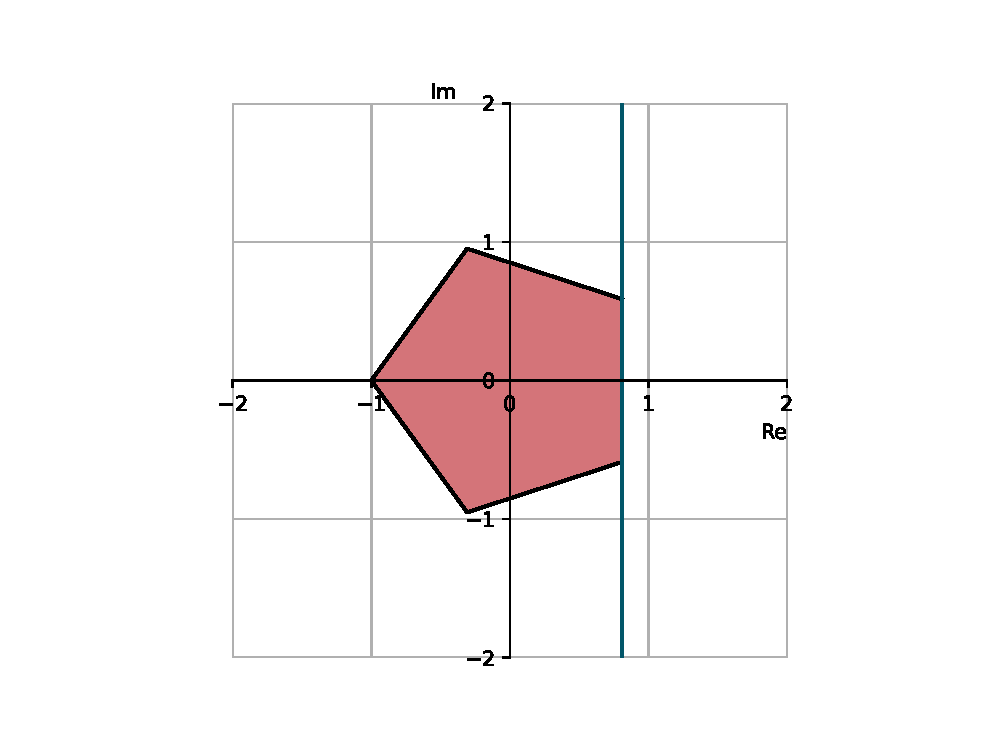
\includegraphics{tetraeder.eps}
	\end{figure}
	Dieses Beispiel orientiert sich an \parencite[S. 146]{gustafson1997numerical}
\end{ex}

\begin{rem} \label{rem:nr_herm}
	Für hermitesche Matrizen stimmen Spektralradius und Operatornorm überein, daher folgt aus Theorem Korollar \ref{cor:norm_num_rad} und \ref{thm:norm_equiv} auch Gleichheit für den numerischen Radius und der Operatornorm:
	\begin{align}
		\rho(A) = w(A) = \|A\|
	\end{align}
	für $A \in Mat_{n,n}(\mathbb{C})$ hermitesch \parencite[vgl. ][S. 266]{goldberg1982numerical} .
\end{rem}

Den zugehörigen Imaginärteil eines Punktes kann man nun leicht mithilfe eines Eigenvektors bestimmen:

\begin{lem} \label{lem:nr_complex}
	Sei $A \in \operatorname{Mat}_{n,n}(\mathbb{C})$, $H_A$ der hermitesche Teil von $A$, $\lambda_g$ der größte Eigenwert von $H_A$ und $v$ ein zugehöriger normierter Eigenvektoren.  Dann \phantom{..} liegt $z=\left< Av,v \right>$ auf der numerischen Abszisse von $W(A)$ und $z \in W(A)$.
\end{lem}
\begin{proof}
	Nach Definition von $z$ gilt bereits: \begin{align}
		z=\left< Av,v \right> = \left< H_A v,v \right> + i \left< S_Av,v \right> = \left< \lambda_g v,v \right> + i \left< S_Av,v \right> = \lambda_g + i \left< S_Av,v \right>
	\end{align}
	Da $\|v\|=1$, gilt also schon $z \in W(A)$. Mit Bemerkung \ref{rem:max_re_nr} folgt die Aussage.
\end{proof}

Die von Johnson beschriebene Methode zur numerischen Approximation des numerischen Wertebereichs aus \parencite{johnson1978numerical} besteht nun darin, einen Punkt auf dem Rand des numerischen Wertebereichs in der gauß'schen Zahlenebene zu bestimmen. Weiterhin kann man zeigen, dass eine Rotation des numerischen Wertebereichs um den Ursprung einer Rotation der ursprünglichen Matrix entspricht. Dadurch können sukzessive alle Punkte auf dem Rand des numerischen Wertebereichs bestimmt werden. Aufgrund der Konvexität und Kompaktheit im Endlichdimensionalen entspricht die konvexe Hülle des Randes genau dem numerischen Wertebereich.

\begin{cor}
	Sei $A \in \operatorname{Mat}_{n,n}(\mathbb{C})$. Dann gilt für alle $\theta \in \mathbb{R}$ \begin{align*}
		e^{i\theta} W(A)=W(e^{i\theta}A),
	\end{align*}das heißt eine Rotation von $W(A)$ um den Winkel $\theta$ entspricht einer skalaren Multiplikation von $A$ mit $e^{i\theta}$. 
\end{cor}
\begin{proof}
	Die Aussage folgt direkt aus Proposition \ref{prop:properties_numran}.
\end{proof}

Für jede Rotation wählt man nun einen einfach zu berechnenden Punkt, beispielsweise einen Punkt auf der numerischen Abszisse des numerischen Wertebereichs in der komplexen Zahlenebene. Von diesem kann man den Realteil mithilfe der beiden Lemmata \ref{lem:nr_real_matrix} und \ref{lem:nr_herm} leicht berechnen. Den zugehörigen Imaginärteil eines Punktes auf dem Rand des numerischen Wertebereichs kann man mithilfe von Lemma \ref{lem:nr_complex} berechnen. Falls die numerische Abszisse den numerischen Wertebereich in mehr als einem Punkt schneidet, reicht es tatsächlich schon aus einen zu kennen. Die restlichen Punkte liegen dann nämlich bereits auf der konvexen Hülle der Punkte \parencite[vgl. ][Theorem 3]{johnson1978numerical}

Unter Ausnutzung der vorherigen Lemmata, Korollare und Bemerkungen hat Johnson einen Algorithmus zur numerischen Approximation des numerischen Wertebereichs entwickelt. Für die Visualisierungen in dieser Arbeit genügt uns schon eine vereinfachte Variante des Algorithmus'.

\begin{algorithm}
	\caption{}\label{euclid}
	\hspace*{\algorithmicindent}\textbf{Input} Matrix $A$, Iterationsschritte $s$\\
	\hspace*{\algorithmicindent}\textbf{Output} $s$ Punkte auf dem Rand von $W(A)$ \\
	
	\begin{algorithmic}[1]
		\For{$k:=0,...,s-1$}
			\State $\theta^{(k)} \gets \frac{2\pi}{s}k$ , $R^{(k)} \gets e^{i\theta^{(k)}}A$ 
			\Comment{\parbox[t]{.4\linewidth}{\footnotesize Winkel und rotierte Matrix initialisieren}} \\
			\State $H_{R^{(k)}} \gets \frac{1}{2}(R^{(k)}+{R^{(k)}}^*)$ 
			\Comment{\parbox[t]{.4\linewidth}{\footnotesize hermiteschen Teil von $R^{(k)}$ berechnen}} \\
			\State $\lambda_g^{(k)} \gets \max_{\lambda \in \sigma(H_{R^{(k)}})} \lambda$
			\Comment{\parbox[t]{.4\linewidth}{\footnotesize größten Eigenwert von $H_{R^{(k)}}$ berechnen}}
			\State $v^{(k)} \gets$ \text{normierter Eigenvektor zu} $\lambda_g^{(k)}$ 
			\Comment{\parbox[t]{.4\linewidth}{\footnotesize zugehörigen normierten Eigenvektoren berechnen}} \\
			\State $z^{(k)} \gets \lambda_g^{(k)} + i \left< Av^{(k)},v^{(k)} \right>$
			\Comment{\parbox[t]{.4\linewidth}{\footnotesize Punkt auf dem Rand von $W(A)$ berechnen}}
		\EndFor \\
		\Return $z^{(0)}, ..., z^{(s-1)}$
	\end{algorithmic}
\end{algorithm}

Damit wurde das Problem auf einzelne, numerisch effizient zu berechnende Eigenwert-Probleme reduziert.

\begin{ex}
	Mithilfe des Algorithmus 1 berechnen wir den numerischen Wertebereich von einigen komplizierteren Matrizen
	\begin{enumerate}
		\item Sei 
		\begin{align}
			A_1 = \begin{pmatrix}
				0.3 & 0.4 & 0.3 \\
				0 & 0.5 & 0.5 \\
				0.7 & 0.1 & 0.2
			\end{pmatrix}
		\end{align}
		\begin{figure}[H]
			\caption{Der numerische Wertebereich von $A_1$}
			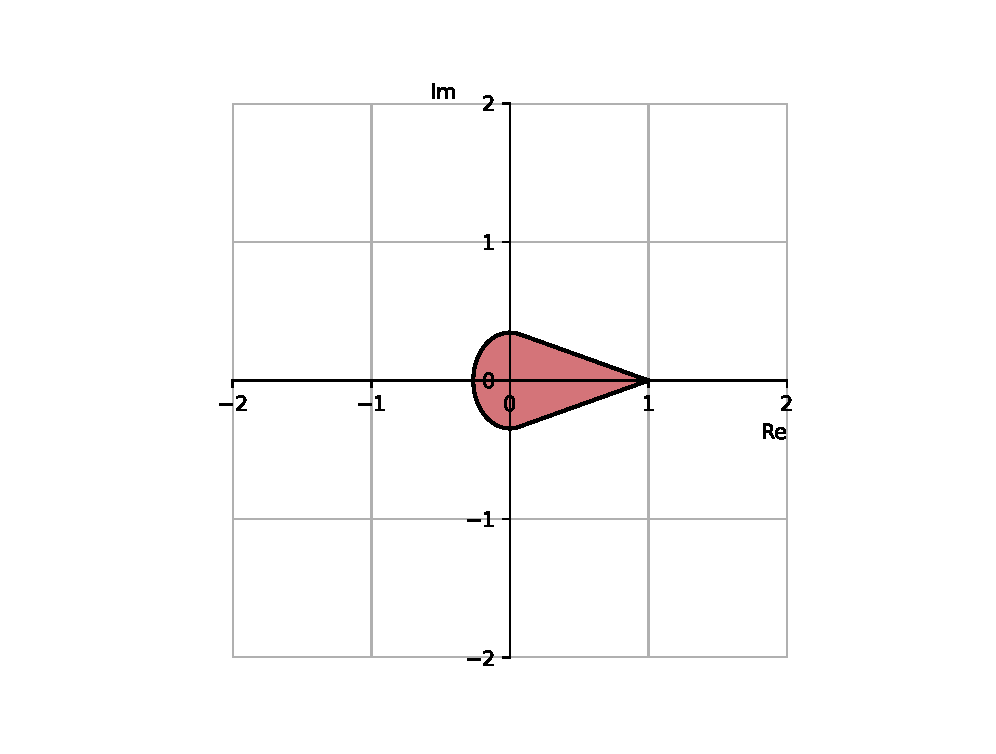
\includegraphics{kegel.eps}
		\end{figure}
		Dieses Beispiel ist entnommen aus \parencite*[S. 601]{johnson1978numerical}
		
		\item Sei 
		\begin{align}
			A_2 = \begin{pmatrix}
				0&0&0&1&0&0 \\ 
				0&0&0&0&0&0 \\
				1&0&0&0&0&0 \\
				0&0&1&0&0&0 \\
				0&1&0&0&0&0 \\
				0&0&0&0&1&0
			\end{pmatrix}
		\end{align}
		\begin{figure}[H]
			\caption{Der numerische Wertebereich von $A_2$}
			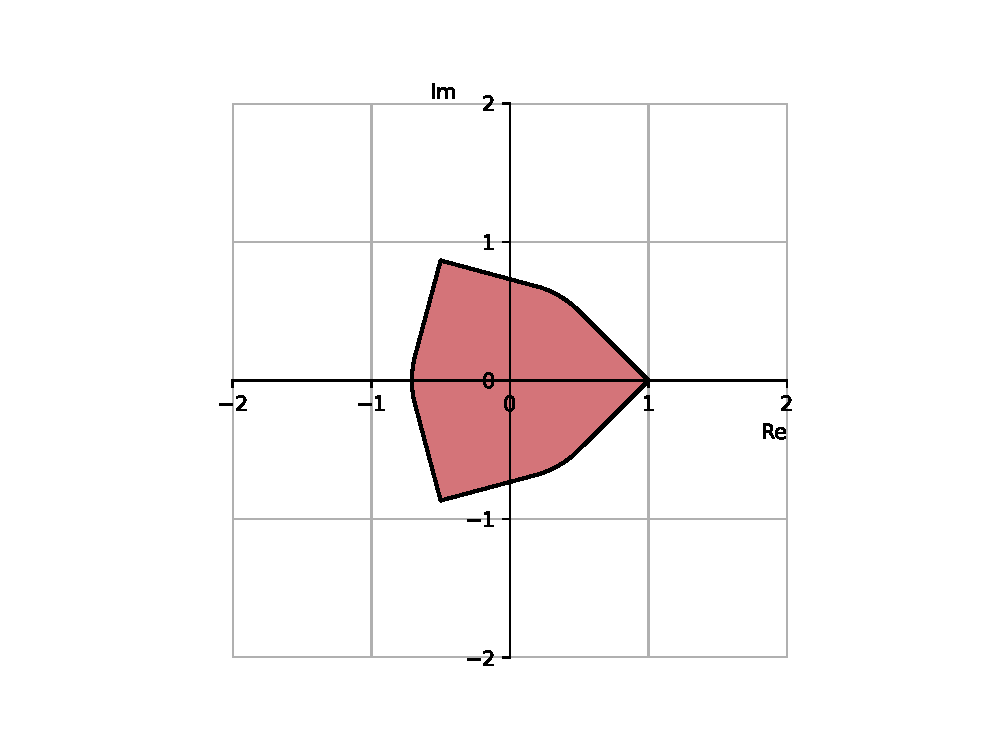
\includegraphics{curved_tri.eps}
		\end{figure}
		Dieses Beispiel ist entnommen aus \parencite*[S. 147]{gustafson1997numerical}
	\end{enumerate}
\end{ex}


